% **************************************************
% Document Class Definition
% **************************************************
\documentclass[%
    paper=A4,               % paper size --> A4 is default in Germany
    twoside=true,           % onesite or twoside printing
    openright,              % doublepage cleaning ends up right side
    parskip=half,           % spacing value / method for paragraphs
    chapterprefix=true,     % prefix for chapter marks
    11pt,                   % font size
    headings=normal,        % size of headings
    bibliography=totoc,     % include bib in toc
    listof=totoc,           % include listof entries in toc
    titlepage=on,           % own page for each title page
    captions=tableabove,    % display table captions above the float env
    chapterprefix=false,    % do not display a prefix for chapters
    appendixprefix=false,    % but display a prefix for appendix chapter
    draft=false,            % value for draft version
]{scrreprt}%

\usepackage{graphicx}

\usepackage{caption}
\usepackage[list=true, listformat=simple]{subcaption}
\makeatletter
\g@addto@macro\p@subfigure{.}
\makeatother

\usepackage{amsmath, amssymb, amsthm, minted, color}

\definecolor{bg}{rgb}{0.95, 0.95, 0.95}
\renewcommand{\theFancyVerbLine}{\sffamily
\textcolor[rgb]{0.5,0.5,1.0}{\scriptsize
\oldstylenums{\arabic{FancyVerbLine}}}}



% **************************************************
% Setup YOUR thesis document in this file !
% **************************************************
% !TEX root = my-thesis.tex


% **************************************************
% Files' Character Encoding
% **************************************************
\PassOptionsToPackage{utf8}{inputenc}
\usepackage{inputenc}


% **************************************************
% Information and Commands for Reuse
% **************************************************
\newcommand{\thesisTitle}{Visualization of biological molecules in web browsers via three.js}
\newcommand{\thesisName}{Pascal Günter Pfannes}
\newcommand{\thesisSubject}{Bachelor Thesis}
\newcommand{\thesisDate}{October 31, 2022}
\newcommand{\thesisVersion}{CleanThesis 0.4.1 - JGU patches}

\newcommand{\thesisFirstReviewer}{Elmar Schömer}
\newcommand{\thesisFirstReviewerUniversity}{\protect{Johannes Gutenberg University Mainz}}
\newcommand{\thesisFirstReviewerDepartment}{Department of Computational Geometry}

\newcommand{\thesisSecondReviewer}{Andreas Hildebrandt}
\newcommand{\thesisSecondReviewerUniversity}{\protect{Johannes Gutenberg University Mainz}}
\newcommand{\thesisSecondReviewerDepartment}{Department of Scientific Computing and Bioinformatics}

\newcommand{\thesisFirstSupervisor}{Elmar Schömer}
\newcommand{\thesisSecondSupervisor}{Thomas Kemmer}

\newcommand{\thesisUniversity}{\protect{Johannes Gutenberg University Mainz}}
\newcommand{\thesisUniversityDepartment}{FB08}
\newcommand{\thesisUniversityInstitute}{Institute of Computer Science}
\newcommand{\thesisUniversityGroup}{Computational Geometry}
\newcommand{\thesisUniversityCity}{Mainz}
\newcommand{\thesisUniversityStreetAddress}{Staudingerweg 9}
\newcommand{\thesisUniversityPostalCode}{55128}


% **************************************************
% Debug LaTeX Information
% **************************************************
%\listfiles


% **************************************************
% Load and Configure Packages
% **************************************************
\usepackage[english]{babel} % babel system, adjust the language of the content
\PassOptionsToPackage{% setup clean thesis style
    figuresep=colon,%
    hangfigurecaption=false,%
    hangsection=true,%
    hangsubsection=true,%
    sansserif=false,%
    configurelistings=true,%
    colorize=full,%
    colortheme=jgured,%
    configurebiblatex=true,%
    bibsys=biber,%
    bibfile=bib-refs,%
    bibstyle=numeric,%
    bibsorting=nty,%
}{cleanthesis}
\usepackage{cleanthesis}

\hypersetup{% setup the hyperref-package options
    pdftitle={\thesisTitle},    %   - title (PDF meta)
    pdfsubject={\thesisSubject},%   - subject (PDF meta)
    pdfauthor={\thesisName},    %   - author (PDF meta)
    plainpages=false,           %   -
    colorlinks=false,           %   - colorize links?
    pdfborder={0 0 0},          %   -
    breaklinks=true,            %   - allow line break inside links
    bookmarksnumbered=true,     %
    bookmarksopen=true          %
}

% **************************************************
% Other Packages
% **************************************************
\usepackage{scrhack}


% **************************************************
% Document CONTENT
% **************************************************
\begin{document}

% uncomment the following command to fill up pages with
% whitespace instead of aligning the first and last lines
% of a page (see \raggedbottom vs. \flushbottom)
%\raggedbottom

% --------------------------
% rename document parts
% --------------------------

% > set short label names for floating environments figure and table
%\renewcaptionname{ngerman}{\figurename}{Abb.}
%\renewcaptionname{ngerman}{\tablename}{Tab.}
\renewcaptionname{english}{\figurename}{Fig.}
\renewcaptionname{english}{\tablename}{Tab.}

% > rename the title of the LOL, i.e. list of listings (default is "Listings")
\renewcommand*{\lstlistlistingname}{List of Listings}

% --------------------------
% Front matter
% --------------------------
\pagenumbering{roman}			% roman page numbing (invisible for empty page style)
\pagestyle{empty}				% no header or footers
% !TEX root = ../my-thesis.tex
%
% ------------------------------------  --> cover title page
\begin{titlepage}
	\pdfbookmark[0]{Cover}{Cover}
	\flushright
	\hfill
	\vfill
	{\LARGE\thesisTitle \par}
	\rule[5pt]{\textwidth}{.4pt} \par
	{\Large\thesisName}
	\vfill
	\textit{\large\thesisDate} \\
	Version: \thesisVersion
\end{titlepage}


% ------------------------------------  --> main title page
\begin{titlepage}
	\pdfbookmark[0]{Titlepage}{Titlepage}
	\tgherosfont
	\centering

	{\Large \thesisUniversity} \\[4mm]
	
\includegraphics[width=6cm]{gfx/jgu_logo_kasten} \\[2mm]
	\textsf{\thesisUniversityDepartment} \\
	\textsf{\thesisUniversityInstitute} \\
	\textsf{\thesisUniversityGroup} \\

	\vfill
	{\large \thesisSubject} \\[5mm]
	{\LARGE \color{ctcolortitle}\textbf{\thesisTitle} \\[10mm]}
	{\Large \thesisName} \\

	\vfill
	\begin{minipage}[t]{.27\textwidth}
		\raggedleft
		\textit{1. Reviewer}
	\end{minipage}
	\hspace*{15pt}
	\begin{minipage}[t]{.65\textwidth}
		{\Large \thesisFirstReviewer} \\
	  	{\small \thesisFirstReviewerDepartment} \\[-1mm]
		{\small \thesisFirstReviewerUniversity}
	\end{minipage} \\[5mm]
	\begin{minipage}[t]{.27\textwidth}
		\raggedleft
		\textit{2. Reviewer}
	\end{minipage}
	\hspace*{15pt}
	\begin{minipage}[t]{.65\textwidth}
		{\Large \thesisSecondReviewer} \\
	  	{\small \thesisSecondReviewerDepartment} \\[-1mm]
		{\small \thesisSecondReviewerUniversity}
	\end{minipage} \\[10mm]
	\begin{minipage}[t]{.27\textwidth}
		\raggedleft
		\textit{Supervisors}
	\end{minipage}
	\hspace*{15pt}
	\begin{minipage}[t]{.65\textwidth}
		\thesisFirstSupervisor\ and \thesisSecondSupervisor
	\end{minipage} \\[10mm]

	\thesisDate \\

\end{titlepage}


% ------------------------------------  --> lower title back for single page layout
\hfill
\vfill
{
	\small
	\textbf{\thesisName} \\
	\textit{\thesisTitle} \\
	\thesisSubject, \thesisDate \\
	Reviewers: \thesisFirstReviewer\ and \thesisSecondReviewer \\
	Supervisors: \thesisFirstSupervisor\ and \thesisSecondSupervisor \\[1.5em]
	\textbf{\thesisUniversity} \\
	\textit{\thesisUniversityGroup} \\
	\thesisUniversityInstitute \\
	\thesisUniversityDepartment \\
	\thesisUniversityStreetAddress \\
	\thesisUniversityPostalCode\ \thesisUniversityCity
}
		% INCLUDE: all titlepages
\cleardoublepage

\pagestyle{plain}				% display just page numbers
% !TEX root = ../my-thesis.tex
%
\pdfbookmark[0]{Abstract}{Abstract}
\addchap*{Abstract}
\label{sec:abstract}

Molecule visualisation software is widely used in the research of biological structures. They offer various models for representing structures as well as means of interacting with them. There is a wide variety of tools available which specialise on certain aspects of molecular research in the form of desktop applications, but also as web-based visualisation software. The main problem of those tools is that the majority of them are not extensible on the user's end. If they need features the tool which they currently use cannot offer they have to find a new application. This results in users having to learn several tools at once. In this thesis we present the \textit{Molecule Visualizer}, a visualisation framework that is supposed to be embedded into \textit{BiochemicalAlgorithms.jl}, a project aiming to re-implement the functionality of BALLView inside a web-based application. The \textit{Molecule Visualizer} provides functionality for visualising molecules in different representations as well as interacting with them. Due to its object-oriented nature we laid the foundation of an extensible visualisation interface in case users need additional functionalities.

\vspace*{20mm}

{\usekomafont{chapter}Abstract}
\label{sec:abstract-diff}

Molekulare Visualisierungssoftware ist weit verbreitet bei der Untersuchung von biologischen Strukturen. Sie bieten die Möglichkeit, Strukturen in verschiedenen Repräsentationen zu betrachten sowie mit ihnen zu interagieren. Es existiert eine große Vielfalt and Software sowohl als Desktopapplikation als auch web-basierte Software, die sich auf bestimmte Bereiche der molekularen Forschung spezialisiert haben. Deren Hauptproblem jedoch ist, dass sie sich auf Seiten der Benutzer nich erweitern lassen. Falls ein Benutzer weitere Funktionalität benötigt, dann muss sich dieser eine neue Applikation suchen. Das hat zur Folge, dass sich Benutzer unter Umständen mit mehreren Tools auf einmal auseinandersetzen müssen. In dieser Arbeit präsentieren wir den \textit{Molecule Visualizer}, ein Visualisierungsframework welches in \textit{BiochemicalAlgorithms.jl} integriert werden soll. Der \textit{Molecule Visualizer} stellt Funktionalitäten zur Verfügung, um Moleküle in verschiedenen Repräsentationen darzustellen sowie mit ihnen zu interagieren. Aufgrund seiner objektorientierten Natur bietet er eine gute Grundlage, um auf Seiten der Benutzer erweitert zu werden, falls weitere Funktionalität benötigt wird, die \textit{BiochemicalAlgorithms.jl} nicht bietet.		% INCLUDE: the abstracts (english and german)
\cleardoublepage
%
\currentpdfbookmark{\contentsname}{toc}
\setcounter{tocdepth}{2}		% define depth of toc
\tableofcontents				% display table of contents
\cleardoublepage

% --------------------------
% Body matter
% --------------------------
\pagenumbering{arabic}			% arabic page numbering
\setcounter{page}{1}			% set page counter
\pagestyle{scrheadings}			% header and footer style

%% Uncomment the following lines using the \part command
%% to add part sections
%\part{Example Part}
% !TEX root = ../my-thesis.tex
%
\chapter{Introduction}
\label{sec:intro}

\section{Motivation}
\label{sec:intro:motivation}

The ability to visualise biological structures and conduct simulations with them is a major breakthrough in the field of molecular biology. Scientists would commit themselves for several years studying a singular structure and construct a model for it by hand before applications for computational visualisation were developed \cite{OLSON20183997, 10.1038/nmeth.1427}. Not only was this a lengthy process, but it could also be hindersome for research until the molecule model had been finished. In order to accurately make predictions about the behaviour of molecules in certain situations like chemical reactions or protein-protein docking you need to understand their structure thoroughly first. After the first visualisation applications had been developed the fields of molecular biology and computational graphics continued to work together and enhanced the technologies used for structural analysis and synthesis \ref{OLSON20183997}. Nowadays, there is a vast amount of tools on the market used for not only molecular visualisation, but also other specialised tasks such as docking simulations for proteins, molecule editors for drug design and many more. The problem is that many of those applications only support basic visualisation functionalities such as different molecule models, basic interaction with molecules and loading biological structures from files without being able to be extended on the user's end if they need more specific features. This leads to development of tools that cover said features which in turn increases the multitude of applications to choose from. 

A solution to this problem would be to develop an application which not only provides basic visualisation and interaction functionalities, but also a way to extend the tool on the user's end. A piece of software that promises extensibility and ease-of-use is called BALLView \cite{10.1093/bioinformatics/bti818, 10.1007/s10822-005-9027-x}. BALLView was developed in C++ with an object-oriented and generic approach by Hildebrandt et al. It is a popular tool for molecule visualisation and modelling. Among the other functionalities that BALLView supports are the calculation of nuclear magnetic resonance spectra, search for structural similarities, molecular mechanics, solvent methods and support for importing or exporting files in various formats. Hildebrandt et al. added the possibility to extend the application by embedding scripts written in Python. Due to outdated dependencies and the majorities of the files being more than ten years old, Hildebrandt and his current research group at the Johannes Gutenberg University in Mainz decided to implement BALLView and its framework again from scratch using the Julia programming language. The project is called \textit{BiochemicalAlgorithms.jl} and aims for recreating the features of BALLView and transform it into a web-based visualisation application. The reason for that is to become platform independent. Instead of developing tools for specific Operating Systems (OS) you create applications that run in web browsers which in turn are available on every OS. Rendering big biological structures is also not a problem as web applications are able to leverage the Graphics Processing Unit (GPU) through the use of a library called WebGL \cite{BibEntry2011Jul}. 

The goal of our project is to provide the visualisation framework for \textit{BiochemicalAlgorithms.jl}, called \textit{Molecule Visualizer}. In order to keep it extensible and easy-to-use, we also follow an object-oriented approach. Communication between the different classes is managed by using events or object references if necessary. This way we ensure that functionalities will be grouped in their own respective class as well as decoupling objects by reducing dependencies between classes. As for basic features it supports visualisation of different molecule models like Ball and Stick, Wireframe or Space-Filling, loading of various molecule structure files and basic interaction involving picking atoms, transforming the molecule or changing atom colors. Instead of using WebGL as our main rendering engine we integrated a package called three.js \cite{BibEntry2022Oct} in our project. three.js is a general-purpose 3D library that supports renderer frameworks for WebGL, Spaced Vector Graphics (SVG) or Cascading Style Sheets 3D (CSS3D). Another major feature is the visualisation of molecules inside a Virtual Reality (VR) environment. The WebXR \cite{BibEntry2022Aug} Application Programming Interface (API) is used to create said environment by communicating with the VR device in order to render molecules on its display and leveraging the device's movement tracking capabilities for interactions with the VR environment. Our project can be found at the following URL: \url{https://gitlab.rlp.net/ppfannes/bachelor_thesis/-/tree/develop}.

\section{Thesis Structure}
\label{sec:intro:structure}

\textbf{Chapter \ref{sec:related}} \\[0.2em]
In this chapter we will provide an overview of important works that were relevant for our project. We include popular web-based tools that inspired us regarding functionalities that we implemented as well as discuss the advantages and disadvantages of web frameworks in general. Desktop software also play an important role in molecular research so we included some applications in order to highlight the differences between web-based and desktop tools.

\textbf{Chapter \ref{sec:visualconcepts}} \\[0.2em]
Important concepts of visualisation will be explained in this chapter as well as the main framework of our application, three.js. A demo program will be used throughout the chapter to explain how the different concepts are realised in three.js. Using the demo we also want to further illustrate our decision to use three.js in our project instead of WebGL.

\textbf{Chapter \ref{sec:implementation}} \\[0.2em]
The basic structure of our project and its core features will be discussed in this chapter. Using various code snippets we are going to explain the rendering process within our tool and how the different components interact with each other.

\textbf{Chapter \ref{sec:evaluation}} \\[0.2em]
In order to gain insight on how our tool fares against existing software we perform an an experiment to evaluate the various applications regarding two important aspects, user-friendliness and functionalities. The results of this experiment will give us the opportunity to categorise our project among other tools and gauge its utility to the bioinformatics community.

\textbf{Chapter \ref{sec:conclusion}} \\[0.2em]
In chapter six we will summarise the results of our project and give an outlook on what functionalities can be added in the future to the \textit{Molecule Visualizer}.
   % INCLUDE: introduction
% !TEX root = ../my-thesis.tex
%
\chapter{Related Work}
\label{sec:related}

The visualisation of molecules and larger proteins is an essential part of molecular biology. It provides the means to conduct further analysis of a molecule's structure and other experiments such as simulations of proteins docking together or drug design. Proper analysis also requires some form of interaction with the visualised object such as changing its representation or editing its structure. As such various tools have been developed over time to take on those tasks and help with research. Even though they all share the same core functionality, i.e. visualisation and basic interactions with the visualised object, the different tools offer a wide variety of intermediate functionality for analysing biological structures. Available software for molecular visualisation can be broadly categorised into two groups: desktop-based and web-based applications. 


\section{Web-based applications}
\label{sec:related:web}

Web-based visualisation tools offer the advantage that only a modern web browser, e.g. Mozilla Firefox or Google Chrome, is necessary in order to use them. This results in a great amount of flexibility as the applications run platform-independent. Deployment and testing of software becomes a much easier task as all you need is a web browser which can be easily installed on the OS of your choice. It is not necessary to emulate a specific OS to check for compatibility for your application. Another advantage is the direct support of mobile devices. Web-based molecule visualisation tools are in general JavaScript libraries that can be embedded into an Hyper Text Markup Language (HTML) web page. Thus, any device capable of displaying web pages can also use web-based visualisation tools. Among the popular choices for web-based molecule visualisation are MolView \cite{Bergwerf2022Oct}, 3Dmol.js \cite{10.1093/bioinformatics/btu829}, and BALLView.

MolView was first released in 2014 and is an open-source molecule visualisation and editing tool. It is based on JavaScript and utilises WebGL + HTML5 to render objects in a web browser. MolView offers a wide range of functionalities from editing options (e.g. add/remove atoms or bonds) over different molecule representations to miscellaneous options, provided through an embedding of JSmol, like molecule measurements, energy calculations and surface representations of electrostatic potentials. It is also possible to search for specific molecules in big databases like the RCSB Protein Data Bank, PubChem Compounds or the Crystallography Open Database by simply specifying the name of the molecule in question. However, biological structures cannot be imported from local files which can pose a problem if none of the used databases contain an entry for a molecule of interest. 

3Dmol.js, initially released in 2015, was developed in JavaScript only and specialises in the visualisation of molecules. There are several ways how 3Dmol.js can be used, either from a JavaScript file, as an embedded viewer in HTML or publicly as a hosted viewer. The diversity in use cases allows 3Dmol.js to be used by not only programmers, but also web developers or even people without programming background. Molecules can be loaded either from local files or by inputting their ID within the PDB. Hardware acceleration as well as parallelised computation of molecular surfaces allow the user to efficiently view and interact with even complex scenes. The developers chose an object-oriented approach for 3Dmol.js so that it can be used in combination with other tools that provide more chemical information regarding the visualised molecule.

Our goal is to provide a visualisation tool that will be integrated into the Biochemical Algorithms Library (BALL) by Andreas Hildebrandt et al. BALL's development started in 1996 as a tool for protein-protein docking, but it quickly grew into a much bigger application supporting various functionalities such as molecule and surface visualisation, loading of multiple molecules at once, several molecular representations and modelling features. All these features are packed into their standalone viewer based on BALL, BALLView. The main goal of the developers was to create a robust and easy-to-use tool for visualising biochemical structures and drug design. For this purpose the application was designed to implement all the functionalities necessary to properly support users during their research. However, they also made sure that it is possible to easily extend the software in case more specified features are needed by the user. Currently, Andreas Hildebrandt and his team are trying to completely reimplement BALL in Julia as the original software depends on old and outdated libraries like OpenGL 1.3. The project is called \textit{BiochemicalAlgorithms.jl} and can be found at the following URL: \url{https://github.com/hildebrandtlab/BiochemicalAlgorithms.jl}.

\section{Desktop applications}
\label{sec:related:desktop}

Desktop software runs directly on the OS of your system which makes them powerful tools. Through OpenGL and the use of shaders the tools communicate with graphics hardware in order to render objects. Operating directly on the OS enables visualisation software to access the various components of the PC and thus leveraging them to address even complex tasks such as simulations or the calculation of molecular surfaces. The major downside to this approach though is the inflexibility of the software. Support for multiple OS requires additional efforts from the developers which could be used to enhance the quality of the product. Additionally, users might not be able to use the software at all if it is not available for their OS which further complicates researches.

Jmol \cite{BibEntry2022Mar} is an open-source Java application for viewing and editing molecules. It started development in the early 2000s and has become one of the most used visualisation tools. It does not depend on WebGL or hardware to render molecules on screen but rather on a framework solely designed for Jmol called z-buffer. To integrate Jmol into other Java applications or web browsers the developers created dedicated components: JSmol which allows for integration into web browsers and JmolViewer which can be embedded in other applications. It also features cross-platform support for Windows, Mac OS X and Linux/Unix systems. Jmol supports a wide range of data formats molecules can be loaded from as well as functionalities for animations, molecule measurements, surfaces and many more.

One of the most used desktop applications for molecule visualisation is PyMOL \cite{PyMOL}. It was initially released in 2000 by Warren Lyford DeLano as an open-source project under the Python License. His ambition was to demonstrate the impact of open-source software on scientific researches by distributing the source code for PyMOL publicly. After his death, Schrödinger Inc. acquired PyMOL in 2010 and since then it has grown into a system with various features not only for molecule visualisation, but also for simulations or drug design. Among different molecule representations, calculation of surface models and tools for animations there is also the possibility to load biochemical structures from local files or via their molecule ID. Instead of a menu bar at the top of the application window PyMOL offers a second window that acts as a command line tool. From there you can perform your manipulations of the displayed object in the main window. The Python interface of PyMOL supports the deployment of additional plug-ins and execution of scripts.   % INCLUDE: related work

%\part{Additional Example Part}
% !TEX root = ../my-thesis.tex
%

\chapter{Visualization Concepts}
\label{sec:visualconcepts}

In this chapter we start by giving an introduction to the main framework used in our application, three.js, followed by an explanation of the core visualisation concepts used in the project. We are also going to explain why we chose three.js over WebGL for our project by constructing and analysing a small demo for both frameworks. The task in the demo is to visualise a coloured and rotating three-dimensional cube. Each major concept mentioned in this chapter is incorporated in the demo. We will refer back to it at the end of each section and illustrate the differences between the two frameworks. This way we want to illustrate why three.js is the better choice for developing a molecule visualisation application. The demo code can be found in our project repository at \url{https://gitlab.rlp.net/ppfannes/bachelor_thesis/-/tree/develop/Research/thesis_examples}.

\section{three.js}
\label{sec:visualconcepts:three}

three.js (formerly known as three.as) is a multi-purpose, open-source 3D JavaScript library written by mrdoob. The aim of three.js is to pose as a general framework for 3D tasks such as visualisation, animation and many more \cite{mrdoob2022Oct}. Additionally, each functionality or component should be designed in a way that does not rely on third-party libraries. In order to achieve those goals three.js is easily extensible in case a new way of rendering is discovered or new components have to be added. As such it provides basic implementations of mathematical structures needed like vectors, matrices as well as other core features for visualisation like Buffers, Objects, Geometries and Uniforms. In addition there are also features for animating, file and object loading, integrating audio tracks and many more. 

To take a closer look at how visualisation works in three.js we will inspect the piece of code shown in snippet \ref{sec:visualconcepts:three:toyscene}.

\begin{listing}[H]
	\begin{minted}[autogobble, bgcolor=bg, breaklines, linenos]{javascript}
	const scene = new THREE.Scene();
	const camera = new THREE.PerspectiveCamera(75, window.innerWidth / window.innerHeight, 0.1, 1000);

	const renderer = new THREE.WebGLRenderer();
	renderer.setSize(window.innerWidth / window.innerHeight);
	document.body.append(renderer.domElement);

	const geometry = new THREE.BoxGeometry(1, 1, 1);
	const material = new THREE.MeshBasicMaterial({color: 0x00FF00});
	const cube = new THREE.Mesh(geometry, material);
	scene.add(cube);

	camera.position.z = 5;

	function animate() {
		requestAnimationFrame(animate);
	
		cube.rotation.x += 0.01;
		cube.rotation.y += 0.01;
	
		renderer.render(scene, camera);
	};

	animate();
	\end{minted}
	\caption{Creation of a small scene in three.js. The scene contains a rotating and coloured cube.}
	\label{sec:visualconcepts:three:toyscene}
\end{listing}
Setting up visualisation in three.js works by first creating a \textit{Scene} and \textit{Camera} object. The \textit{Scene} acts as a container where all the objects that should be rendered will be added to. The \textit{Camera} defines the field of view in which you can see the rendered objects. Next up is the initialisation of the renderer used, in this case a \textit{WebGLRenderer}. It acts as an API which abstracts away most of WebGL's functionalities and leaves the user with a set of core functions to render objects. This allows developers to focus more on the development of their application instead of having to invest a decent amount of time creating visualisations with purely WebGL. Especially if the project features various representations of objects as it is the case with our \textit{Molecule Visualizer}. After the renderer has been initialised the cube will be created in lines 8-10. In three.js objects are represented as meshes that consist of a Geometry describing the shape of the object and a material describing its outward appearance. The cube is then added to the \textit{Scene} and is now ready to be rendered which will be done in the animate function. Lines 16-19 make the cube rotate around the x and y-axis while the actual rendering takes place in line 21. Using the \textit{Scene} and the \textit{Camera} the renderer visualises the cube on the screen within the field of view of the camera. To actually see the output of this code it has to either be embedded into an HTML file directly or you need to reference the source file containing the code. Both methods are shown in snippet \ref{sec:visualconcepts:three:threeembedding}.

\begin{listing}[H]
	\begin{minted}[autogobble, bgcolor=bg, breaklines, linenos]{html}
	<!-- Method 1: Embed source code directly into the HTML page. -->
	...
	<script src="path/to/three.js"></script>
	<script>
		<!-- visualisation code here... -->
	</script>
	...
	
	<!-- Method 2: Specify path to the source code file. -->
	...
	<script src="path/to/visualisation/source/file"></script>
	...
	\end{minted}
	\caption{Methods of embedding three.js code into a web page to see the visualisation.}
	\label{sec:visualconcepts:three:threeembedding}
\end{listing}

\section{Meshes}
\label{sec:visualconcepts:meshes}

Meshes are used to model complex structures like living beings or geometrical objects. They are constructed by approximating the surface of objects using triangles. Instead of calculating them directly while rendering they are implicitly defined via the positions of their corners, also called vertices. The connection between a pair of vertices is called edge and they are used to keep track of all vertices that make up a triangle, also called face. Those three components, vertices, edges and faces, are the main components that construct a mesh. Additionally you can also define further properties that change the appearance of the mesh like materials or UV Coordinates. During the render pipeline in the graphics hardware shaders are used to help building a concrete mesh. Materials define regions in the mesh that use a different shader than the rest which results in a changed appearance of the area. UV Coordinates also influence the later outward appearance of a mesh by specifying which parts of a two-dimensional texture map are applied to which part of a mesh. UV Coordinates can be considered a mapping of the two-dimensional texture space to the three-dimensional coordinate space of the mesh. Each vertex is assigned a pixel of the texture map that will later be rendered on the vertex's position.

\begin{listing}[H]
\begin{minted}[autogobble, bgcolor=bg, breaklines, linenos]{javascript}
// WebGL mesh creation.
...
function initBuffers(gl) {
	const posBuffer = gl.createBuffer();
	gl.bindBuffer(gl.ARRAY_BUFFER, posBuffer);
	const vertices = [...];
	gl.bufferData(gl.ARRAY_BUFFER, new Float32Array(vertices), gl.STATIC_DRAW);
	...
	const colBuffer = gl.createBuffer();
	gl.bindBuffer(gl.ARRAY_BUFFER, colBuffer);
	gl.bufferData(gl.ARRAY_BUFFER, new Float32Array(colors), gl.STATIC_DRAW);
	
	const indBuffer = gl.createBuffer();
   	gl.bindBuffer(gl.ELEMENT_ARRAY_BUFFER, indBuffer);
   	const indices = new Uint16Array([...]);
   	gl.bufferData(gl.ELEMENT_ARRAY_BUFFER, indices, gl.STATIC_DRAW);
   	...
}
...
\end{minted}
\begin{minted}[autogobble, bgcolor=bg, breaklines, linenos]{javascript}
	// three.js mesh creation.		
	const boxGeometry = new THREE.BoxGeometry(boxWidth, boxHeight, boxDepth);
	const boxMaterials = [...];   // Array of MeshBasicMaterial instances.
	const box = new THREE.Mesh(boxGeometry, boxMaterials);
\end{minted}
\caption{Mesh creation in WebGL vs. three.js. WebGL needs to initialise buffer objects for vertex positions, colors and face indices and bind them in order to prepare a mesh. three.js only has to create instances for the object's geometry and material to create meshes.}
	\label{sec:visualconcepts:meshes:meshinitex}
\end{listing}

To get a better understanding of how mesh creation works we will take a look at how both WebGL and three.js handle this task. The code snippets in listing \ref{sec:visualconcepts:meshes:meshinitex} show the process of mesh creation for WebGL and three.js respectively. As one can see, it takes farm more lines of code (LOC) to produce a mesh in WebGL than in three.js. To be able to create a mesh in WebGL you need to first define the positions of the vertices followed by the colours of the various Faces. Both the positions and colours are then bound to buffer objects which will allow WebGL to pass multiple values to the shaders during rendering. The last step is the creation of an index array which defines the vertices that make up a face.

Defining a mesh in three.js only requires the geometry of the object and the material used to alter its appearance which are already provided as base classes, \textit{BufferGeometry} and \textit{Material}. \textit{BufferGeometries} act as a container for different attributes regarding meshes like Vertex positions, Face normals or UV Coordinates as well as custom attributes. Attributes are stored similarly to WebGL. Lines 7, 11 and 16 show that the attribute information is stored by writing it to the corresponding buffer that was bound previously using \textit{gl.bindBuffer}. The arrays have to be converted to typed JavaScript arrays before they can be saved. Instead of only using typed JavaScript arrays \textit{BufferGeometries} use a wrapper class and the corresponding typed array to store attribute information (e.g. \textit{Float32BufferAttributes} for \textit{Float32Arrays}). In the case of the \textit{BoxGeometry} class according to the width, height and depth provided in the constructor the geometry of a box with those parameters will be created in the background. \textit{Materials} contain information regarding the appearance of the object to be rendered. Attributes are stored as properties of the \textit{Material} instance to keep it independent from the renderer framework used. The \textit{Mesh} class ultimately acts as a container for both the geometry information as well as the appearance information of objects. Compared to WebGL, three.js abstracts away the creation of geometry attributes and material properties by introducing classes that handle these tasks upon instantiation.

\section{Camera}
\label{sec:visualconcepts:camera}

In order to visualise the mesh of a three-dimensional object as a two-dimensional image its vertex coordinates need to be transformed. This transformation is referred to as \textit{Projection} and describes the process of mapping the vertex positions to points within the two-dimensional image plane. A series of matrix multiplications is used to transform vertex coordinates where each matrix plays a different role during transformation. This can be seen in figure \ref{sec:visualconcepts:camera:transform}. The first step involves transforming the vertex coordinates from object to world space using the model matrix. It is able to manipulate objects by altering their position, rotation and size. After that the world space coordinates need to be transformed with respect to the camera. This is achieved by applying the view matrix which can be expressed as the inverse of the camera's model matrix. The final transformation step involves the projection matrix which contains information about the camera's field of view. Applying the projection matrix ensures that only coordinates within the camera's field of view will be rendered, effectively discarding all other coordinates. There are two types of projection matrices, each yielding a different result when applied. The perspective projection matrix creates an output that is similar to how the human eye perceives objects. The further away an object is the smaller it will be rendered. Applying an orthographic projection matrix yields an image that has no depth information at all. Every object in the field of view of the camera will appear to have the same depth value. The figure also shows that some steps can be combined to gain performance by applying less matrix multiplications.

\begin{figure}[htb]
	\centering
	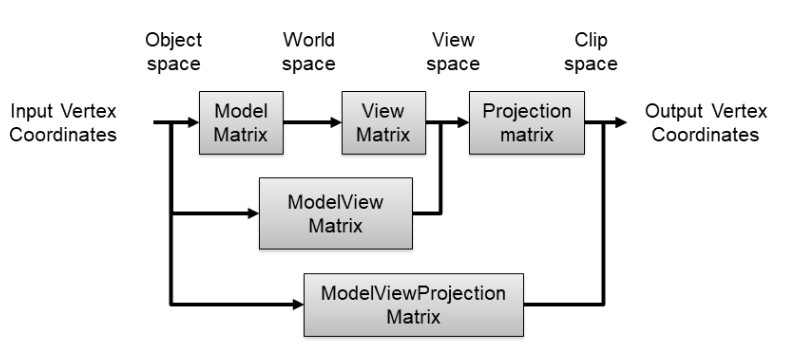
\includegraphics[width=\textwidth]{gfx/transformations.jpg}
	\caption[Transformation of vertex coordinates to image plane coordinates.]{Transformation of vertex coordinates to image plane coordinates\footnotemark.}
	\label{sec:visualconcepts:camera:transform}
\end{figure}
\footnotetext{https://www.doc.ic.ac.uk/~bkainz/graphics/notes/GraphicsNotes0405.pdf; accessed on 31 October 2022}

Listing \ref{sec:visualconcepts:camera:cameraex} shows how the camera is manipulated in WebGL and three.js. The projection matrix has to be explicitly created in WebGL by first defining the fov, aspect ratio, near and far plane and then applying those values on an empty matrix (lines 5-11). The model-view Matrix is treated similarly. First you create an empty matrix and the you apply the transformations on it that will alter the object's position and rotation during rendering. For the transformations to take effect, the matrices need to be stored in their respective Uniforms so the shaders have access to them. In three.js you create an instance of the \textit{PerspectiveCamera} class in order to manipulate objects. The parameters passed to its constructor are the same that are used to create the projection matrix in WebGL. Instead of directly working with the matrices, you manipulate the object directly and inside the \textit{renderer.render} function the Projection and model-view matrices will be updated. This approach seems a bit more intuitive, because you apply the transformation directly to the object and the matrices are updated during rendering instead of the other way around like WebGL does. You can also see that everything regarding the matrices which transform objects is abstracted away through the \textit{renderer.render} function.

\begin{listing}[H]
\begin{minted}[autogobble, bgcolor=bg, breaklines, linenos]{javascript}
// WebGL camera.
...
function sceneDraw(gl, progInfo, buffers, deltaTime) {
	...
    glMatrix.mat4.perspective(projMatrix, fov, aspect, near, far);

    const modelViewMatrix = glMatrix.mat4.create();
    glMatrix.mat4.translate(modelViewMatrix, modelViewMatrix, new Float32Array([0.0, 0.0, -4.0]));
    glMatrix.mat4.rotateZ(modelViewMatrix, modelViewMatrix, cubeRotation);
    glMatrix.mat4.rotateY(modelViewMatrix, modelViewMatrix, cubeRotation * 0.7);
    glMatrix.mat4.rotateX(modelViewMatrix, modelViewMatrix, cubeRotation * 0.3);
   	...
   	gl.uniformMatrix4fv(progInfo.uniformLocs.projMatrix, false, projMatrix);
    gl.uniformMatrix4fv(progInfo.uniformLocs.modelViewMatrix, false, modelViewMatrix);
   	...
}
...
\end{minted}
\begin{minted}[autogobble, bgcolor=bg, breaklines, linenos]{javascript}
// three.js camera.		
const camera = new THREE.PerspectiveCamera(50, canvas.clientWidth / canvas.clientHeight, 0.1, 100);
camera.position.z = 3.5;
...
time *= 0.001;
    
box.rotation.z = time;
box.rotation.y = time * 0.7;
box.rotation.x = time * 0.3;
    
renderer.render(scene, camera);
...
\end{minted}
\caption{Camera manipulation in WebGL vs. three.js. While you have to directly change the projection and model-view matrix in WebGL you only have to transform objects in three.js The camera will be adjusted in the \textit{renderer.render} function.}
\label{sec:visualconcepts:camera:cameraex}
\end{listing}

\section{Raycasting}
\label{sec:visualconcepts:raycasting}

As the name implies \textit{Raycasting} uses rays that are cast from the focal point to detect and render objects. For every pixel that will be generated on the Image Plane a ray is generated and traced until all intersections with objects in the world space are found. The first intersection found determines which object will be rendered on the corresponding pixel of the image plane. Another useful application of \textit{Raycasting} is \textit{object picking}. By casting the ray from the mouse pointer's position instead of the focal point and stopping after finding the first intersection one can determine if the mouse pointer is currently hovering over an object.

\section{Virtual Reality}
\label{sec:visualconcepts:virtualreality}

\textit{Virtual Reality} (VR) is the simulation of a world either similar to the real world or different from it. VR offers various degrees of immersion into the simulated surroundings such as visual immersion, motion tracking or full body immersion \cite{10.3389/fpsyg.2018.02086}. There are several types and methods as well including simulation-based, projector-based, desktop-based or VR via head-mounted devices (HMD). Projector-based simulations are used for applications in which it is necessary to have an accurate and realistic representation of the real world. Examples would be construction modelling, robot navigation or airplane simulation. Whereas in simulation-based VR the surroundings rendered can be made-up.  The key point is generating an experience as if the user is truly present in the virtual world by providing realistic feedback based on the user's inputs. This can be seen in many simulation games where one is driving a vehicle or operating a machine. Desktop-based VR involves displaying a three-dimensional world on a regular display without the use of other devices connected to VR such as lenses or motion-tracking devices. Instead the feeling of immersion is created by using various triggers or responsive characters. HMDs consists of two small displays inside the device that render the environment for each eye separately. This enables stereoscopic vision that results in a more realistic experience of the surroundings. A binaural sound system as well as motion tracking of the head enhance this experience even further. Motion controls or an omnidirectional treadmill to allow for realistic movement and interactions within the virtual world are optional.

Incorporating VR into web applications poses a problem, because of the wide range of devices on the market all supporting different degrees of movement, controls and position tracking. That is why in 2016 \textit{WebVR} was introduced as a first attempt of creating a general API for web based VR applications \cite{BibEntry2018Sep, WebVRIntro}. It featured full support for VR headsets, motion and position tracking as well as a Gamepad interface for controller support. WebVR made it possible to more easily develop VR applications without the developers being concerned about supporting multiple devices, because it serves as an abstraction of the devices' hardware. While it posed as a great start to web-based VR development it was only an experimental API and it soon became apparent that a new framework needed to be created. This led to the introduction of \textit{WebXR} two years later in 2018 \cite{BibEntry2022Jul}. One key difference is the support for \textit{Extended Reality} (XR) meaning Augmented Reality (AR) and VR. Another difference is the controller support for some VR devices. Instead of leveraging the existing Gamepad interface WebXR offers an own implementation along with events that are responsible for squeeze and select controls.

All applications build with the WebXR API follow a similar life cycle \cite{BibEntry2022Aug}. The first code snippet in listing \ref{sec:visualconcepts:virtualreality:vrex} illustrates said cycle and how it can be implemented in WebGL. At first you have to request a session from \textit{navigator.xr} and set the mode in which the VR session should be started in. After the session has been set successfully, the returned Promise will be resolved in which the \textit{xrReferenceSpace} will be set up. The reference space is responsible for setting up the movement tracking environment within a VR scene. There are different modes for the \textit{xrReferenceSpace} which make assumptions about the user's movement from the initial starting point in the scene as well as in the environment in general and thus adjust the stability of the tracking space. Then you need to make sure that the WebGL context used to render the normal scene is now set up to render the VR environment. This is done by calling \textit{gl.makeXRCompatible}. Once the render context is updated you need to update the render state and frame buffer as well. Doing so will tell the WebXR API where to render the contents of the VR scene to. Now that the set up for the \textit{xrSession} is complete the only thing left is to set up a render loop for the scene. The callback is defined similarly to a normal scene with the exception that it now also takes a second parameter which is an \textit{xrFrame}. The \textit{xrFrame} object is responsible for saving the state of all tracked objects within a VR scene. You are able to retrieve the viewer pose from an \textit{xrFrame} which is needed for rendering the scene to both lenses of an HMD. By calling \textit{xrSession.requestAnimationFrame} you register the render callback in the same way as in a non-VR scene.

The rendering process of a VR scene is similar to that of a non-VR one with the exception that the scene has to be rendered multiple times, one for each view matrix in the viewer pose. Each view matrix represents the transformations associated with the lens of a VR device and the Projection as well as the Model-View Matrix are constructed with respect to it (lines 27 and 28 of the first snippet). To ensure that the scene has been rendered for all devices registered in the \textit{xrSession}, \textit{gl.finish} is called in line 22 of the first snippet. This function waits until all previously called WebGL functions have been completed.
The above process has been drastically abstracted in three.js as seen in code snippet two. In order to create a VR scene one has to import the \textit{VRButton.js} file which initiates the \textit{xrSession} after being clicked. Then you need to tell the renderer you want to enable VR by setting the \textit{renderer.xr.enabled} flag to \textit{true}. \textit{renderer.xr} is an instance of the WebXRManager class which manages essentially everything about the VR environment, e.g. session set-up, input devices, device cameras or updating of components during VR rendering. To create the animation loop in three.js you call the \textit{renderer.setAnimationLoop} method and provide the render function as an argument. \textit{setAnimationLoop} accomplishes the same result as \textit{xrSession.requestAnimationFrame} by registering the render function within the \textit{WebXRManager} to be called during visualisation. 
When dealing with VR applications three.js provides an API that abstracts a big part of the set-up usually needed for them. As one can see in the first code snippet, you would normally need to set up the entire session as well as the render environment yourself while in three.js you only need a few small changes to the source code to create a stable VR application. 
\begin{listing}[H]
\begin{minted}[autogobble, bgcolor=bg, breaklines, linenos]{javascript}
// WebGL VR scene.
...
function enterVR() {
	navigator.xr.requestSession('immersive-vr').then((session) => {
	// Set up xrReferenceSpace.
	inVR = true;

	gl.makeXRCompatible().then((xrContext) => {
		// Set up render state and frame buffer.
	});

	const renderVR = (now, frame) => {
		// Similar to render with the exception of setting up xrFrame; call to sceneDrawVR with same parameters as in non-VR.
	};

	xrSession.requestAnimationFrame(renderVR);
	});
}
...
function sceneDrawVR(gl, progInfo, buffer, deltaTime) {
	// Same setup as in sceneDraw; retrieve pose of xrFrame so you can render the scene for each eye of the VR headset.
	gl.finish();
}
...
function renderEye(gl, progInfo, buffers, eye) {
	// Set up Projection and View Matrix with respect to the eye that is currently rendered; rest of function like sceneDraw.
	projection = eye.projectionMatrix;
	view = eye.transform.inverse.matrix;
	...
}
...
\end{minted}
\begin{minted}[autogobble, bgcolor=bg, breaklines, linenos]{javascript}
// three.js VR scene.
// import VRButton.js for setting up xrSession.
...
renderer.xr.enabled = true;
document.body.appendChild(VRButton.createButton(renderer));
...
renderer.setAnimationLoop(render);
\end{minted}
\caption{VR setup in WebGL vs three.js. A lot of setup is required in order to set up a VR scene for WebGL. All the functionality for setting up VR in three.js is abstracted away in \textit{VRButton} and \textit{renderer.xr}.}
\label{sec:visualconcepts:virtualreality:vrex}
\end{listing}       % INCLUDE: concepts
% !TEX root = ../my-thesis.tex
%

\chapter{Implementation}
\label{sec:implementation}

\begin{figure}[htb]
	\centering
	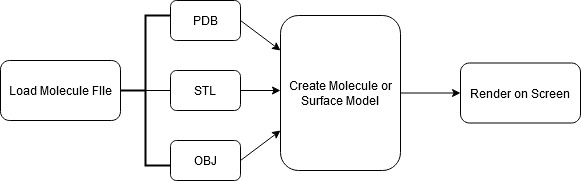
\includegraphics[width=\textwidth]{gfx/visualisation_pipeline.jpg}
	\caption{Visualisation Pipeline.}
	\label{sec:implementation:vispipe}
\end{figure}

Figure \ref{sec:implementation:vispipe} shows the general visualisation pipeline of the \textit{Molecule Visualizer}. After selecting a new molecule to display the \textit{loadFile()} event is responsible for determining which \textit{Molecule Representation} was used and extracting the file's content. The structure of the extracted content depends on the representation used and the corresponding loader provided by three.js. According to the information provided by the loaders the molecule model is generated and rendered afterwards. The following sections will detail the process of visualisation and describe the different molecule models and molecule representations supported by the \textit{Molecule Visualizer}. Before that we will outline the structure of our project and how the different classes are connected. Furthermore the communication between the Graphical User Interface (GUI) and the Visualizer is going to be discussed. Currently, they communicate with each other via the use of events which are managed by a global instance of the \textit{EventManager} class. Lastly, the use and application of VR in our application will be explored. We decided to only include minimal interaction possibilities during the VR session and no GUI for changing the displayed molecule or its representation. Here we will explain our reasoning as to why we did this.

\section{Overview}
\label{sec:implementation:overview}

In order to create our visualisation application we decided to follow an object-oriented approach. Reason for that is the goal of designing a tool that can easily be extended and has interchangeable components. This has the advantage that one can create new objects that inherit from our classes and add new functionalities without much effort. We also managed to minimise dependencies between objects by grouping together functions that perform similar tasks, i.e. all visualisation-related functions belong to one class, all GUI-related functions belong to a class etc. If two classes need to communicate with each other this can be achieved by either storing an instance of the object in question or by using event-based communication. We preferred to use Event communication as often as we could, because it helps decoupling objects and prevent unnecessary dependencies.

\begin{listing}[H]
\begin{minted}[autogobble, bgcolor=bg, breaklines, linenos]{javascript}
// Constant section.
const NEAR = 1e-6;
const FAR = 2000;
const scene = new THREE.Scene();
const camera = new THREE.PerspectiveCamera(50, innerWidth / innerHeight, NEAR, FAR);
const container = document.getElementById('container');
const renderer = new THREE.WebGLRenderer({canvas: container, antialias: true, logarithmicDepthBuffer: true});
const stats = new Stats();
const cameraGroup = new THREE.Group();
const prevGamePads = new Map();
let cameraVector = new THREE.Vector3();
let speedFactor = [0.1, 0.1, 0.1, 0.1];
let frontLight1, frontLight2, backLight1, backLight2;
// Properties section.
class Visualizer {
	constructor() {
		this.root = new THREE.Group();
		this.controls = new TrackballControls(camera, renderer.domElement);
		this.objectPicker = new ObjectPicker(this.root, camera);
		this.moleculeModel = new Model();
		this.renderRequested = false;
		this.debugGUI = new VisualizerGUI();
		this.moleculestruct = {};
		this.modal = new Modal(document.querySelector('#modal'));
		this.changedAtomColor = new Map();
	}
}	
\end{minted}
\caption{Structure of the \textit{Visualizer} class.}
\label{sec:implementation:overview:visualizer}
\end{listing}

The \textit{Visualizer} class contains the main functionality of our tool. Each of the other classes is connected to it via Event-based communication to trigger changes in the visualisation. Code snippet \ref{sec:implementation:overview:visualizer} shows the general structure of \textit{Visualizer}. The class has references to the other classes in order to create event functions that should be triggered once the corresponding functionality has been triggered. As the \textit{Visualizer} acts as the main part of our application it also keeps references to render-related objects like \textit{scene}, \textit{camera} or \textit{renderer}. Rendering has been realised using render-on-demand which means that we only want to render when something about the representation of the molecule changed like the model or atom colors. This increases the performance of the application and saves resources by calling the render routine only when necessary. During rendering we use a special kind of meshes to increase performance called \textit{InstancedMesh}. They work just like normal mesh objects in three.js, but they also require an \textit{instanceCount} parameter that specifies how many instances of this mesh should be rendered. That means you can render multiple objects in one render call. As previously mentioned, the \textit{Visualizer} also sets up the Event functions that should be called when their associated functionality is triggered. For example changing the rendered molecule if you chose a new file via the GUI. This is done by first defining the Event function and then registering it in the \textit{EventManager} class by calling \textit{EventManager.addEvents}.

\begin{listing}[H]
\begin{minted}[autogobble, bgcolor=bg, breaklines, linenos]{javascript}
// Properties section.
class EventManager extends EventDispatcher {
	constructor() {
		this.managedEvents = new Map();
	}
}

// Example of how to add event listeners to objects.
EventManager.addEvents(object, [event1, event2, ...], [eventFunction1, eventFunction2, ...]);

// This is how objects and events are stored internally.
{object: {event1: eventFunction1,
          event2: eventFunction2,
          ...},
}
\end{minted}
\caption{Structure and usage example of the \textit{EventManager} class. In order to add event listeners to objects you have to provide a reference to the object, a list of events and a list of corresponding event functions. Note that event and function have to have the same position in their respective arrays in order to store them correctly.}
\label{sec:implementation:overview:eventmanager}
\end{listing}

In order for our classes to communicate with each other we created the \textit{EventManager} class. This class is responsible for managing events and the corresponding listener objects. This way we are able to freely add and remove events any time necessary. Code snippet \ref{sec:implementation:overview:eventmanager} shows the structure of the \textit{EventManager} and an example of how to use the object. You are able to add multiple events to an object by calling \textit{EventManager.addEvents}. In order to manage the objects we store them inside a map with the object being the key and the value being another object containing the added events and their corresponding functions. The structure of the map is also illustrated in code snippet \ref{sec:implementation:overview:eventmanager}.

The \textit{ObjectPicker} class is responsible for interacting with the rendered molecules in the normal scene as well as in the VR environment. A raycaster is used to cast a ray from the mouse position and detect if you clicked an atom or not. Clicking atoms informs the \textit{Visualizer} class to show a modal containing information about the atom like its position or color. Inside the VR scene a ray is cast from the controller's position instead and checked for intersections with atoms.

\begin{listing}[H]
\begin{minted}[autogobble, bgcolor=bg, breaklines, linenos]{javascript}
// Create GUI structure.
const api = {
	button: () => {	// Buttons are defined via callbacks.
		...
	},
	checkbox: false	// Checkboxes are defined via booleans.
	dropdown: {	// Drop-down menus are defined by listing the options within an object.
		...
	},
	color: 0x00Ff00,	// Colors are defined by using their hexadecimal representation.
	input: '',	// Input fields are defined by using a string literal.
	
	// Create GUI folder where gui is the GUI to add the folder to.
	const folder = gui.addFolder('folder');
	// Add GUI element to folder. In this case we add a button to the GUI.
	folder.add(api, 'button');
};
\end{minted}
\caption{Example of how to define and bind GUI elements.}
\label{sec:implementation:overview:visualizergui}
\end{listing}

Our GUI is defined inside the \textit{VisualizerGUI} class. It is closely connected to the \textit{Visualizer} class by sending events every time a setting has been changed. We inherited from the GUI class of three.js to generate the interface and manage our settings. The GUI consists of folders in which you can add elements like buttons or checkboxes. Code snippet \ref{sec:implementation:overview:visualizergui} illustrates the process of adding elements to the GUI. First you create the structure of the GUI as a JavaScript object. Depending on the content of its entries the added elements will differ, e.g. buttons are defined as functions inside the structure object. Then you create a folder for the GUI and add the element to it by referencing the structure object and the corresponding field name.

Showing atom information after clicking them is handled by the \textit{Modal} class. It receives a reference to an HTML element that should act as the modal body and will be populated by the \textit{Modal} class. After an atom has been clicked the content of the modal window will be constructed and then set via the \textit{Modal.setModalContent} method. Closing the modal can be done by clicking on its close button or clicking anywhere on the browser window. Currently modals are only available after loading molecules from Protein Data Bank (PDB) files as they provide atom information like periodic table symbol or color after parsing them. 

The \textit{Model} class handles management of the currently chosen molecule model and the corresponding mesh(es). It is also responsible for creating them in the first place. After loading a molecule or choosing another representation the \textit{Model} class is tasked with (re-)rendering the molecule according to the chosen representation. 

\section{Molecule Representation}
\label{sec:implementation:molrepr}

The first part of the visualisation pipeline is determining which type of molecule file is loaded and extracting its contents. Each file type stores various pieces of information regarding the molecule's composition and structures them differently. Currently, our Molecule Visualizer supports three different formats of molecule files: PDB, Wavefront .obj \cite{article} (OBJ) and Stereo Lithography \cite{BibEntry2019Sep} (STL). While PDB files only store the position of the atoms within the molecule OBJ and STL files store the coordinates of all vertices and faces that form the mesh. In the following two sections we are going to discuss the properties of the previously mentioned file formats as well as their advantages and disadvantages. Lastly, we will elaborate on their use case and how such files are handled within our application.

\subsection{Standard Representation}
\label{sec:implementation:molrepr:pdb}

The PDB file format is used for describing the structure of molecules that are included in the Protein Data Bank. It is a text-based format which contains information regarding nucleic acids within the molecule, atom positions and their connectivity as well as secondary structures \cite{BibEntry2022Jan}. PDB files have a width limit of 80 columns which stems from its introduction in 1970s. During that time punch cards were used to store data in a portable format and cards with 80 columns were the most commonly used ones \cite{Maxfield2011Oct}. Each line has to start with a specific keyword indicating what type of content to expect e.g. atomic coordinates or information regarding the nucleic acids present.

The most important keywords for our application to be able to render the described molecules are ATOM and CONECT as three.js already provides a loader called \textit{PDBLoader} that is capable of parsing PDB files. With the help of those tags the \textit{PDBLoader} constructs a JSON object which contains three fields: \textit{atomPositions}, \textit{bondPositions} and \textit{json}. The first two entries are \textit{BufferGeometries} that hold the positions of the atoms and bonds (in case of \textit{atomPositions} the atom colors as well). \textit{json} contains atom meta-data regarding position, color and periodic table symbol. This information is displayed inside modals which are triggered after clicking an atom. 

PDB files contain not only information about the basic geometry of the molecule, but also about its Secondary Structures. Secondary Structures occur based on the conformation of the atoms within a protein and are essential for defining a protein's structure \cite{DEGREVE2014384, 10.3389/fbioe.2021.687426}. The two most common types are $\beta$-Sheets and $\alpha$-Helices. In order to visualise those structures it is necessary to know which amino acids take part in forming the $\beta$-Sheets or $\alpha$-Helices which is exactly what PDB files provide. A different loader would be required as the one provided by three.js only parses the ATOM, HETATOM or CONECT lines in the files. This would mean that either the \textit{PDBLoader} has to be extended or another parsing library for PDB files has to be used. As one of our future goals is to integrate the \textit{Molecule Visualizer} into BALL.jl where we leave the molecule file handling to the Julia backend we deemed it not necessary to extend the \textit{PDBLoader} or use an external parser. Furthermore, the use of an external tool would require us to create the \textit{BufferGeometries} for atoms and bonds ourselves while this is already handled by three.js' loader. 

\subsection{Surface Representation}
\label{sec:implementation:molrepr:surface}

PDB files describe molecules in terms of atom positions and which atoms are bonded whereas STL and OBJ files represent their surface as a surface mesh. The surface mesh offers a clearer understanding of a molecule's three-dimensional structure and is also vital for simulations in which you try to dock smaller compounds onto proteins. STL files encode objects as a tessellated two-dimensional surface, i.e. a triangle mesh approximating the objects' surface \cite{SZILVSINAGY2003945}. For each triangle the following information is stored: its normal and the vertex coordinates. There is no information held regarding material or color of the object.

STL files with the \textit{solid} keyword followed by the name of the object. Triangles are stored by first declaring their normal, then each vertex by its coordinates within the mesh. Coordinates have to be represented as floating point numbers following the format sign-mantissa-\textit{e}-exponent. After all triangles have been defined the file ends with the \textit{endsolid} keyword. To ensure the file's validity it has to follow specific rules \cite{HAMANN1994197}. These rules ensure that the content of the STL file is valid and a correct tessellation of the object's surface. In order for the mesh to be connected each triangle should share at least one Vertex with other triangles. To prevent bifurcations an edge should only be shared by at most two triangles. 

OBJ files are able to represent the surface of an object as well. Similar to STL files they save information about the surface mesh by using the vertex coordinates and triangle faces. Additionally, vertex normals are stored as well which enables the use of Smooth Shading techniques such as \textit{Phong Shading}. As a result the rendered surface has a more natural appearance than surfaces generated from STL files. There is also a difference in how face normals are handled. While they are explicitly given for STL models, in OBJ they are inferred from the vertex coordinates as they are given in counter-clockwise order by default \cite{Iqbal2019Sep}.

One major advantage of OBJ files over STL is the realistic appearance of objects due to Smooth Shading and more accurate representation. Curved surfaces also cannot be precisely rendered using triangle meshes which means a loss in accuracy. A solution would be to use more triangles to approximate the curve, but this would result in extremely large STL files. To circumvent this problem, OBJ files are able to leverage techniques such as free-form geometry or surfaces \cite{Iqbal2019Sep}. 

\section{Molecule Models}
\label{sec:implementation:molmodels}

After identifying the type of representation used in the molecule file and parsing its content the actual model has to be created. Depending on the representation the Molecule Visualizer provides various model options to choose from. In total three molecule models are supported: Ball and Sticks, Wireframe and Space-Filling (Van der Waals. Those models are only available after loading a PDB file as STL and OBJ files only provide information for the molecule surface but not about the individual atoms or bonds. Each model presents different advantages regarding molecule properties, e.g. geometry, size, structure and interaction of molecules. We are going to give a short introduction to the models and their purpose in molecule visualization followed by an explanation on how they are implemented in our application.

\subsection{Ball and Stick}
\label{sec:implementation:molmodels:ballstick}

The Ball and Stick model is one of the basic visualisation models for chemical compounds and molecules. Atoms are represented by coloured spheres and bonds as small sticks. This representation is useful for examining the bonds of a molecule as they are explicitly shown and represented with their correct angles. One downside to the model is that it cannot accurately show the relative space covered by the molecule as the bond length compared to the radii of the atoms is made to be longer \cite{Hamzah2022Jul}. The bonds are more visible this way and the model is more simplified at the cost of an exact spacial representation. As such, Ball and Stick models are useful when it comes to analysing atomic bonds and the geometry of larger biological molecules.

We realized the Ball and Stick model in our application with the use of \textit{InstancedMeshes}. As the atoms and bonds only differ in color and scaling we could leverage the ability of \textit{InstanceMeshes} to create multiple objects at once with a single call to the GPU thus increasing visualization performance. Creating the model consists of constructing the atom and bond meshes followed by rendering them on the display. The meshes are built inside a function of the same name as the model. Atom meshes use \textit{IcosahedronGeometry} instead of \textit{SphereGeometry} to appear like spheres as the surface of icosahedrons can be smoothed easier without the direct use of shaders. Increasing the detail and thus the number of vertices effectively transforms the icosahedron into a sphere. Bond meshes use \textit{BoxGeometry} which is scaled and translated during the mesh creation to appear as a thin line connecting the atoms.

Assembly of atoms and bonds is split into their own, separate functions, \textit{createAtoms} and \textit{createBonds}. Both functions work in a similar way as they first construct the transformation matrix for the corresponding object which is applied to it afterwards. This step is repeated \textit{count} times with \textit{count} being the number of instances of the Instanced Mesh. The transformation matrices differ regarding the scale and rotation of the objects, because atoms and bonds require different positioning and orientation in three-dimensional space. While rotation is of no concern for atoms bonds need to be rotated such that they face their corresponding start and end point, i.e. the two spheres forming an atomic bond. Scaling atoms only requires changing their radius. Bonds on the other hand need to be scaled in both width and length to be properly positioned and sized. Editing the transformation of Instanced Meshes proved to be relatively complicated. One is able to access the transformation matrix of each mesh instance, which is represented as a \textit{Matrix4} object, but the matrices do not offer an interface for easily changing individual components without affecting the remaining components. Hence a dummy object is used to determine the correct transformation for every atomic bond. The dummy object is an instance of \textit{Object3D} and treated as a substitute for the bond mesh on which to apply the rotation, scale and translation. \textit{Object3D} provides a proper API such as the \textit{lerp} method for correctly positioning the bond object between atoms and the \textit{lookAt} function which rotates the dummy object so that it connects the atomic centers. Afterwards the transformation matrix of the dummy is extracted and used for the bond mesh. Once the atom and bond meshes have been created they can be added to the scene and the finished model will be rendered.

\subsection{Wireframe}
\label{sec:implementation:molmodels:wire}

Wireframe models consist of the atomic bonds within a molecule rendered as thin lines. The ends are coloured to represent the atoms taking part in a particular bond. Atoms would be placed at the intersection of the lines. Similar to the Ball and Stick model the focus is on the general geometry of a molecule as well as the bonds and their associated angles. The molecular structure is even more abstracted and simplified due to the missing spheres. This enhances the visibility of bonds within bigger biomolecules such as proteins, as there are less distractions. Also, there is no loss of information, because then end of each atomic bond is coloured indicating which atom would normally be at this position.

As atoms are not a part of the Wireframe model we reused the code from the \textit{ballAndStickModel} function and left out the atom creation. The resulting method is called \textit{wireframeModel}. Normally the end of the lines would be coloured to indicate which atom is normally placed there, but this would require a different format as the one the \textit{PDBLoader} class provides. One would have to add an entry to the object returned by the \textit{PDBLoader} which associates every atom position with the index of the corresponding atom in the \textit{json} field. One would use the positions given in the \textit{bondGeometry} field to look up the index of the atom participating in an atomic bond and therefore its color. This works because the coordinates in \textit{bondGeometry} are ordered such that atoms belonging to the same bond have their positions listed one after another.

\subsection{Space-Filling}
\label{sec:implementation:molmodels:vdw}

Space-Filling (or Van der Waals) models are similar to Ball and Stick models with the difference that atom spheres are scaled much bigger, according to their Van der Waals radius. This results in bonds not being visible anymore. The advantage of this model lies in the depiction of space occupied by a molecule. In Ball and Stick models atoms are scaled smaller to make bonds more visible, therefore using less relative space than in reality. Space-Filling representations however visualise atoms using their actual radius to more accurately depict the space a molecule occupies.

Van der Waals models are created using the \textit{createAtoms} function, but with a slight difference. Instead of passing the normal atom radii to the function the Van der Waals radii are used to create the enlarged atoms. Bonds are not visible when using this representation so we dropped the bond creation for increased performance. The result is comparable to the Ball and Sticks representation, but with the difference that bonds are missing and atoms are scaled bigger. This way the space used by the molecule is shown more accurately. 

\section{Communication between Components}
\label{sec:implementation:comm}

After the Molecule Visualizer has finished loading the model file and constructing the respective molecule model it is then rendered on the screen. One final question regarding the Visualisation Pipeline remains: how do the various components of our  application interact with one another to achieve this result? There are two different ways inter-component communication is realized within the \textit{Molecule Visualizer}: through the help of object references and events.

The \textit{Visualizer} class has a reference to all components that make up the application thus having access to all their functionality. As soon as a file has been chosen by the user via the GUI a callback to the \textit{Model} class with the necessary information, i.e. the file and its type, will be initiated to build the molecule model. As choosing a file is functionality that is solely handled by the GUI there has to be a way to transmit information regarding chosen settings or files to the \textit{Visualizer} class. Adding a reference to the \textit{Visualizer} in the \textit{VisualizerGUI} class was discarded quickly as one of our goals was to make the \textit{Molecule Visualizer} a flexible and easily understandable software, i.e. expandable in a simple way as well as having a user-friendly interface that can be grasped quickly. Thus dependencies between components should be kept to a minimum. Using a direct reference to the \textit{Visualizer} class would mean that the functionality for each button in the GUI would have to be explicitly defined as a method that can be called. Increasing the complexity of the GUI would result in a lot of functions that enable communication between the \textit{Visualizer} and \textit{VisualizerGUI} classes. Changing or adding functionality would mean appending or removing methods for communication. All of the aforementioned points lead to a convoluted \textit{Visualizer} class and various dependencies between interface and Visualizer. The same holds for any other component that needs to communicate with the \textit{Visualizer} class. For that reason we decided to use Events as our means of enabling inter-component data exchange with the help of a class called \textit{EventManager}. Events will help us enable communication between GUI an \textit{Visualizer} that does not cause unnecessary dependencies and keeps our software expandable.

The \textit{EventManager} object is used as a global manager for all event-based communication inside our application. It derives from the \textit{EventDispatcher} class in three.js which provides an interface to create event-driven communication and applications. Event communication is based on listening for events and dispatching them. An object needs to have a so-called \textit{EventListener} attached to it so that whenever the corresponding Event is dispatched it will be notified and the function associated with the Event will be executed. It is important to note that only the listeners of the dispatching object are notified instead of listeners from other objects. Thus the \textit{EventListener} needs to be attached to the same object that is used to send the Events out. The \textit{EventManager} supports the attachment of multiple listeners at once by supplying the object which should listen for Events, a list of Event names and an array of Event functions where the ith Event function corresponds to the ith Event name in the list. Adding multiple listeners at once helps to reduce redundancy in the code if an object needs to listen for a lot of events. As soon as the object dispatches an Event it has a listener for the Event function will be executed. 

To set up the inter-component communication we import the \textit{EventManager} class in every component that needs to transmit data to other components. Importing the \textit{EventManager} will import an instance of that class which can be used immediately. Inside the \textit{Visualizer} class we defined a function called \textit{addEvents} which is responsible for defining all Event functions that are used in our application. For each method a constant is defined containing the functionality that should be executed when the Event is dispatched. We divided the Events into multiple categories one of them being Events regarding inter-component communication. Their listeners are attached to the \textit{EventManager}. Before using Events we would resorted to using new class functions for each GUI element that needed to transmit data to the \textit{Visualizer}. Code snippet \ref{sec:implementation:overview:eventmanager} depicts the process of adding new functionality to the GUI using event-based communication. After adding a new element to the interface we define a new constant within the \textit{addEvents} function. The list of Event names and functions are appended with the new Event identifier and constant respectively. Those collections act as parameters for the \textit{addEvents} method of our \textit{EventManager}. Once the listeners are applied to the \textit{EventManager} object we dispatch the Event if the user interacts with the newly added GUI element. 

\section{Visualisation in Virtual Reality}
\label{sec:implementation:visualvr}

The \textit{Molecule Visualizer} is not only able to display molecules on screen as three-dimensional objects, but also in VR with the help of the WebXR interface. We did not have to interact with the API directly, as three.js already offers support of VR by adding an object called \textit{VRButton} to our scene. For this object to work correctly the web browser needs to support WebXR which can be checked by looking for the \textit{xr} property of the navigator variable. If that is not defined VR is not supported and the \textit{Molecule Visualizer} will not be able to display molecules in VR space. Otherwise clicking the button will start the VR application cycle explained in section \ref{sec:visualconcepts:virtualreality}.

Once inside the VR scene the user will immediately be able to see the molecule that was rendered in the browser window before. To properly interact with the object you need to be able to move around and atoms should be clickable. We solved the moving aspect by implementing camera controls with the help of controllers. This means that users do not need enough space around them to inspect the object from various angles, but they can use controllers instead given that their VR headset offers support for them. One uses the analog sticks to move the camera around the object. This is done by querying the controllers registered in the current VR session for which button has been pressed. As moving the camera and the controller models proved to be quite difficult we resorted to using a \textit{Group} object. By adding the aforementioned objects into the \textit{Group} and applying transformations on it, each of its children will be moved as well. Being able to click on atoms requires getting the direction the controller is facing to determine if an object is pointed at. This is done by taking the rotation component of its transformation matrix and applying it to the ray cast by the \textit{Raycaster}. We also set the position of the ray's origin to be the controller's current position within the world and test for any intersections along the ray's path. Once we find an intersection the corresponding atom is highlighted. Clicking it will open up a prompt similar to the modals we used in the non-VR scene. However this prompt is not created using HTML/CSS, because they cannot be displayed inside a VR environment. Instead we rely on a library called \textit{three-mesh-ui} \cite{felixmariotto2022Oct}. It allows the creation of GUI elements which derive from three.js' \textit{Object3D} interface. Doing so enables the usage of said elements within the VR environment by adding them to the scene like a normal object and removing when not needed anymore. This way if an intersection between our controller and an atom exists we add a textbox similar to the modal  The range of GUI elements that are provided by \textit{three-mesh-ui} is limited to boxes, inline boxes, virtual keyboards and text. Creating a functional GUI like in the non-VR scene with those elements poses to be quite a difficult task. As our main focus with this work was to visualize biological structures and molecules we decided to treat the VR environment as another way of inspecting objects without changing their representation or color. To view other representations in VR one would have to change it in the non-VR scene and then click the \textit{VRButton} object to start the session. This is quite cumbersome to do, but the easiest solution given the circumstances. Other frameworks like React360 \cite{facebookarchive2022Oct} or AFrame \cite{aframe} would solve our problem, but integrating them into an existing three.js project is rather challenging as well. It could change in the near future though as there is an extension of the WebXR API planned that supports displaying DOM content within a VR session \cite{immersive-web2022Oct}.         % INCLUDE: system
% !TEX root = ../my-thesis.tex
%

\chapter{Evaluation}
\label{sec:evaluation}


\section{Setup}
\label{sec:evaluation:setup}

\begin{table}[h]
\begin{tabularx}{\textwidth}{ | c | X | }
\hline
Acer Nitro N50-600 & Windows 10 Home, Intel(R) Core(TM) i5-9400 CPU @2.90 GHz, 16GB RAM, NVIDIA GeForce GTX 1060 6GB \\ \hline
Oculus Rift & Inter-Pupillary Distance (IPD): 58-72 mm, Resolution: 1080x1200 per eye, Refresh Rate: 90Hz, Tracking: 6 Degrees of Freedom (6DoF) outside-in (base stations required), Controllers: partial finger tracking via capacitive sensors \\ \hline
\end{tabularx}
\caption{Table containing the specifications of the PC and VR device used during the evaluation.}
\label{sec:evaluation:setup:specstable}
\end{table}

The Molecule Visualizer provides basic functionality for inspecting molecules such as loading different representations, selecting and colouring atom groups as well as changing models during visualization. In this evaluation we want to compare the Molecule Visualizer with other visualization tools and gain insights on how our application can be ranked among them. We decided to choose tools from the following four categories to properly categorize the Molecule Visualizer: web-based + no VR (3Dmol.js, MolView), web-based + VR support (Nanome \cite{nanome}, ProteinVR \cite{10.1371/journal.pcbi.1007747}), web-based on three.js (GLmol \cite{biochem-fan2022Oct}, NGL \cite{10.1093/bioinformatics/bty419, 10.1093/nar/gkv402}) and desktop applications (PyMOL, Jmol). Table \ref{sec:evaluation:setup:specstable} contains the specifications of the PC and the VR device we used for testing. To assess the performance of the different tools and formulate a proper classification we specified two important aspects according to which we will evaluate during our experiment: user-friendliness and functionalities of the application. As we intend our application to be used by other scientists we want to deploy a tool that is easy to use and features the most important aspects necessary for molecular research. The following paragraphs provides a list of functionalities that we expect the applications to have and which qualities make up a user-friendly software.

An application is user-friendly if it meets the following criteria: 
\begin{itemize}
	\item \textbf{Easy-to-grasp GUI}: The interface should be easily understandable by the user. Its structure should help with grasping how the application works, i.e. it should not cause the user to be more confused. For more complex GUIs, a guide should be provided to explain the most essential settings.
	\item \textbf{Documentation}: The developers should provide some sort of documentation for their software, be it within the project repository or as an extra website to explain their application in more detail. The documentation should also be well-maintained an be up-to-date with the most recent version of the software.
	\item \textbf{Setup}: The Setup of the application should be designed so that users without experience in Computer Science are able to install the software on their machine, i.e. it should be accessible to everyone. If necessary, a guide should be provided, either through an installer, on the download page or an entry in the documentation, that explains the necessary steps for the installation.
	\item \textbf{Support}: For further questions or problems Support should be provided in the form of a discussion forum or a contact address that people could send their problems to. 
\end{itemize}

Following functionalities should be part of the examined tools:
\begin{itemize}
	\item \textbf{Molecule Models}: The applications should feature several molecule models especially basic representations like Ball and Stick, Space-Filling and Wireframe in order for researchers to properly investigate the structure of molecules. The more models are supported the better.
	\item \textbf{Loading of various molecule file types}: Molecules should be able to be loaded from a file either locally or from a remote server. If the application is able to calculate molecular surfaces itself then the support for surface files is not needed. 
	\item \textbf{Interactions with molecule}: It should be possible to interact with the visualised molecules. Means of interaction can be versatile such as simple camera movement, selection, editing of the molecule, labelling etc. The more functionalities for interaction are supported the better.
	\item \textbf{Colouring}: Choosing different color schemes for molecules or individual colouring of atoms should be supported as a means to highlight specific regions of interest within a molecule.
\end{itemize}

To determine the existence of the documentation we look for links on the download page of the application or for further links within the tool. As for the web-based software we check the repository of the project for links as well or a README file that documents usage of the application. Its quality will be judged based on several factors: Does it contain a tutorial on basic functionalities and the set-up? Does it document the tools' features? Is it structured properly? Is there a section regarding additional support? 

Tutorials can help to understand the core functionalities of an application quicker and speed up the process of "getting used to the tool". Once the software is big enough and supports enough features users will quickly get overwhelmed with the application's set-up or how to use it properly. That is why the existence of tutorials in a documentation is essential to prevent the user from being confused and frustrated while using the software. The same goes for the set-up process. As for the next two points, the documentation should not only mention the capabilities of the application, but also explain how they work and are used. There should be different sections for each feature and, if necessary, groupings of functionalities that perform similar tasks. Lastly, there has to be a section containing further links to community forums, other help platforms or a developer contact if users need help on problems that are cannot be solved with the help of the documentation. Checking activity of users as well as the developers on these platforms is also a sign of a well-maintained software and indicates if the tool is still in use.

\begin{table}[t!]
\begin{tabularx}{\textwidth}{| X | X | X | X | X |}
\hline
& Easy GUI & Documentation & Support & Set-up \\ \hline
GLmol & + & - & $\sim$ & + \\ \hline
NGL & + & ++ & + & + \\ \hline
3Dmol & + & ++ & + & + \\ \hline
ProteinVR & $\sim$ & ++ & + & + \\ \hline
PyMOL (free) & $\sim$ & $\sim$ & - & - \\ \hline
Jmol & ++ & ++ & ++ & + \\ \hline
Nanome & $\sim$ & ++ & + & + \\ \hline
MolView & ++ & $\sim$ & + & + \\ \hline
Molecule Visualizer & + & $\sim$ & + & + \\ \hline
\end{tabularx}
\caption{Results of User-friendliness evaluation.}
\label{sec:evaluation:benchmark:userfriendeval}
\end{table}

\section{Benchmark}
\label{sec:evaluation:benchmark}

\begin{table}[t!]
\begin{tabularx}{\textwidth}{| X | X | X | X | X | X |}
\hline
& Basic molecule models & Local or remote molecule loading & Various file types supported & Interactions with molecule & Colouring \\ \hline
GLmol & + & ++ & $\sim$ & + & + \\ \hline
NGL & ++ & ++ & ++ & ++ & + \\ \hline
3Dmol & ++ & + & $\varnothing$ & ++ & + \\ \hline
ProteinVR & ++ & ++ & + & ++ & + \\ \hline
PyMOL & ++ & ++ & ++ & ++ & + \\ \hline
Jmol & ++ & ++ & + & ++ & + \\ \hline
Nanome & ++ & ++ & ++ & ++ & + \\ \hline
MolView & ++ & $\sim$ & $\varnothing$ & ++ & + \\ \hline
Molecule Visualizer & + & + & + & + & + \\ \hline
\end{tabularx}
\caption{Results of functionality evaluation.}
\label{sec.evaluation:benchmark:funceval}
\end{table}

Tables \ref{sec:evaluation:benchmark:userfriendeval} and \ref{sec.evaluation:benchmark:funceval} contain the results of our evaluations. As one can see in regards to user-friendliness the results vary drastically between the various applications. For example Jmol's interface is really intuitive for users as the buttons show pop-ups that explain what the button is used for. It has a very detailed documentation page that also contains tutorials on the usage of Jmol. Regarding support there are various forums in which users can post questions and receive help from other Jmol users. Set-up is uncomplicated as well as it only involves downloading the application and following the instructions of the installer. On the other hand, PyMOL has not only an open-source version, but also a licensed version of the tool. We used the open-source version of PyMOL for our evaluation. The set-up of the open-source version is relatively complicated as the instructions on the page that the open-source project refers to are not clear enough to successfully install it. Support is locked behind buying a license for PyMOL, the same goes for the documentation. There are a few tutorials accessible for free, but they refer to older versions of PyMOL. When using PyMOL for the first time the interface is quite overwhelming as it features two separate windows, one visualisation window and a command-line interface. Without a proper tutorial visualising a molecule and performing tasks like changing the color of atoms, changing the representation or even just interacting with the molecule can be quite difficult. Both VR applications, Nanome and ProteinVR, suffer from an initially complicated user interface. This stems from the various functionalities both of them support. Otherwise their documentations are well-structured and feature videos for further explanations. Compared to their rich VR environment the VR scene in our tool is still rather empty and only permits limited interactions with molecules. This is due to the restrictions we faced when trying to set up a GUI in VR. Functionality-wise our application is rather limited. Every one of the tested tools offers functionalities beyond standard representations or basic interactions. ProteinVR and Nanome offer a fully functional VR scene including GUI and advanced controls. MolView, NGL and Jmol offer the ability to edit molecules. Calculating molecular surfaces and additional representations for molecules can be found in all tools.

Compared to the aforementioned tools our Molecule Visualizer can be categorised as a solid alternative. It might not have the support for the amount of features from other applications, but we designed our project with extensibility in mind which was present in almost none of the tested tools. Only PyMOL showed signs of extensibility via Python scripts. Our project also supports the most basic features for molecular research and leaves a lot of room for improvement in the future with additional representations for example. Regarding user-friendliness, our user interface is pretty small due to the limited functionalities, but still clearly structured which becomes harder the more features you support. Our documentations is currently not up-to-date with the current state of our project which will be solved in the near future. Other than that it can be compared to some of the better structured documentations like the one for Jmol or Nanome.	   % INCLUDE: evaluation
% !TEX root = ../my-thesis.tex
%
\chapter{Conclusion}
\label{sec:conclusion}

We presented the \textit{Molecule Visualizer}, a visualisation framework that is capable of rendering molecules in different models and offers basic interaction with the visualised structures. We implemented it as a web-based visualisation tool, because it is easier to exchange research results and the performance of rendering in web browsers has drastically increased with the introduction of WebGL. In order to render objects we used the three.js library instead of WebGL directly, because three.js offers an intuitive API that simplifies mesh creation and rendering. It also provides the means to quickly set up a VR environment without many changes to the render loop. 

Our software is meant to be to be integrated into the \textit{BiochemicalAlgorithms.jl} project by Hildebrandt et al. As they envision their project to be easy-to-use and extensible on the user's end, we tried to design our project around those ideas. We followed an object-oriented approach that encapsulates functionalities in their own classes, e.g. the \textit{ObjectPicker} class for picking objects or the \textit{Model} class for managing molecule models. Reducing dependencies between objects is realised using communication based on events sent between classes. The advantage of an object-based design is that users are later able to add new features by defining new objects which inherit from our base classes. Those objects would then implement the new functionalities the user needs. 

In the end we evaluated our project alongside other visualisation tools regarding their user-friendliness and the different functionalities they support. The \textit{Molecule Visualizer} does not support as many functionalities as the other tools, but it still has a solid foundation which leaves room for improvement. We talk about further additions in section \ref{sec:conclusion:future}. It is also one of the few tools that is built towards extensibility together with PyMOL which supports Python scripts with additional functionalities. Following an object-oriented approach makes it easier for users to either define completely new objects and add them to the \textit{Molecule Visualizer} or add more features to already existing objects. It also helps with integrating our tool into \textit{BiochemicalAlgorithms.jl}. The user-friendliness of our application compared to the other tools is above average. While some projects halted development or do not offer a well-structured documentation the Molecule Visualizer is still being developed and also offers documentation in form of a separate web page. In the future we will address various bugs that could not be solved due to time constraints and add more features to make our tool even more versatile.

\section{Future Work}
\label{sec:conclusion:future}

The features of our \textit{Molecule Visualizer} can be extended by making the following additions:
\begin{itemize}
\item Due to time constraints our project could not be integrated into \textit{BiochemicalAlgorithms.jl} yet. If it were integrated we would be able to add more molecule models like Cartoon. This model gives biological structures a comic-like appearance and is a good choice for visualising proteins. We already added a prototype for the Cartoon model setting which uses Catmull-Rom splines to render a tube given an array of control points. We would replace the current control points with an array containing the positions of $\alpha$-carbon atoms which form the backbone of a protein. The spline would then run through the backbone of the protein, yielding the desired cartoon representation.
\item Currently it is only possible to visualise and interact with molecules inside VR, but there is no GUI for manipulating its appearance or changing models. This is a limitation of the WebXR API. It is not possible to render interactive HTML/CSS directly in a VR scene. This is why we resorted to three-mesh-ui for the modal boxes that appear when you pick an atom. three-mesh-ui only supports a small amount of interactive elements though e.g. buttons or a virtual keyboard. There are no drop-down menus or checkboxes that we use for selecting different models and providing test molecules for visualisation. But there are other alternatives in development like CanvasUI which supports different shapes for textboxes, scrolling text and color selection. Drop-down menus and sliders are in the works. 
\item Another important feature of BALLView besides visualisation is the ability to build peptides. This functionality is especially helpful for drug design where you want to create new active ingredients to cure illnesses. This can be done by changing the instance count of the Instanced Meshes to add or remove atoms and bonds. \textit{BiochemicalAlgorithms.jl} would have to take on the task of making sure the resulting molecule is physically correct, i.e. the bond lengths and angles between the atoms are correct.
\end{itemize}     % INCLUDE: conclusion

% --------------------------
% Back matter
% --------------------------
%
{%
\setstretch{1.1}
\renewcommand{\bibfont}{\normalfont\small}
\setlength{\biblabelsep}{0pt}
\setlength{\bibitemsep}{0.5\baselineskip plus 0.5\baselineskip}
\printbibliography[nottype=online]
\newrefcontext[labelprefix={@}]
\printbibliography[heading=subbibliography,title={Webpages},type=online]
}
\cleardoublepage

\listoffigures
\cleardoublepage

\listoftables
\cleardoublepage

\listoflistings
\cleardoublepage

\cleardoublepage
% !TEX root = ../my-thesis.tex
%
\pagestyle{empty}
\hfill
\vfill
\pdfbookmark[0]{Colophon}{Colophon}
\section*{Colophon}

This thesis was typeset with \LaTeXe.
It uses the \textit{Clean Thesis} style developed by Ricardo Langner.
The design of the \textit{Clean Thesis} style is inspired by user guide documents from Apple Inc.

Download the \textit{Clean Thesis} style at \url{http://cleanthesis.der-ric.de/}.


\cleardoublepage
% !TEX root = ../my-thesis.tex
%
%************************************************
% Declaration
%************************************************
\pdfbookmark[0]{Declaration}{Declaration}
\addchap{Declaration}
\label{sec:declaration}
\thispagestyle{empty}

I hereby declare that I have written the present thesis independently and without use of other than the indicated means. I also declare that to the best of my knowledge all passages taken from published and unpublished sources have been referenced. The paper has not been submitted for evaluation to any other examining authority nor has it been published in any form whatsoever.

\bigskip

\noindent\textit{\thesisUniversityCity, \thesisDate}

\smallskip

\begin{flushright}
	\begin{minipage}{5cm}
		\rule{\textwidth}{1pt}
		\centering\thesisName
	\end{minipage}
\end{flushright}

%*****************************************
%*****************************************

\clearpage

\newpage
\mbox{}

% **************************************************
% End of Document CONTENT
% **************************************************
\end{document}
